\newpage

\section{Simulation Analysis}
\label{sec:simulation}

\subsection{Simple circuit}

\begin{figure}[H]
\centering
\includegraphics[width=0.6\textwidth]{gain_sim}
\caption{Data collected versus simulated data}
\label{data_graph_sim}
\end{figure}

It is obvious, from the above graph, that there are slight deviations between the real data and the simulated data, as expected. This can be due to any number of experimental causes:

\begin{itemize}

\item Errors in the peak to peak amplitude determined by the oscilloscope

\item Errors in the resistors used in the lab (had gold tolerance)

\item Errors in the capacitors used in the lab

\item For the $500\;\Omega$ resistor, two $1\;k\Omega$ resistors were employed, in parallel

\item All signals went through the breadboard

\item $V_{CC}$ was not exactly $10\;V$ and $V_{EE}$ was not exactly $-10\;V$

\item Discrepancies in the {\bf Ngpisce} models

\end{itemize}

Using these parameters, the following was obtained:

\begin{table}[H]
  \centering
  \begin{tabular}{|c|c|}
    \hline
        {\bf Name} & {\bf Value} \\
        \hline
        \hline
        \input{lab}
        \hline
  \end{tabular}
  \caption{Results}
  \label{sim_results}
\end{table}

\begin{figure}[H]
\centering
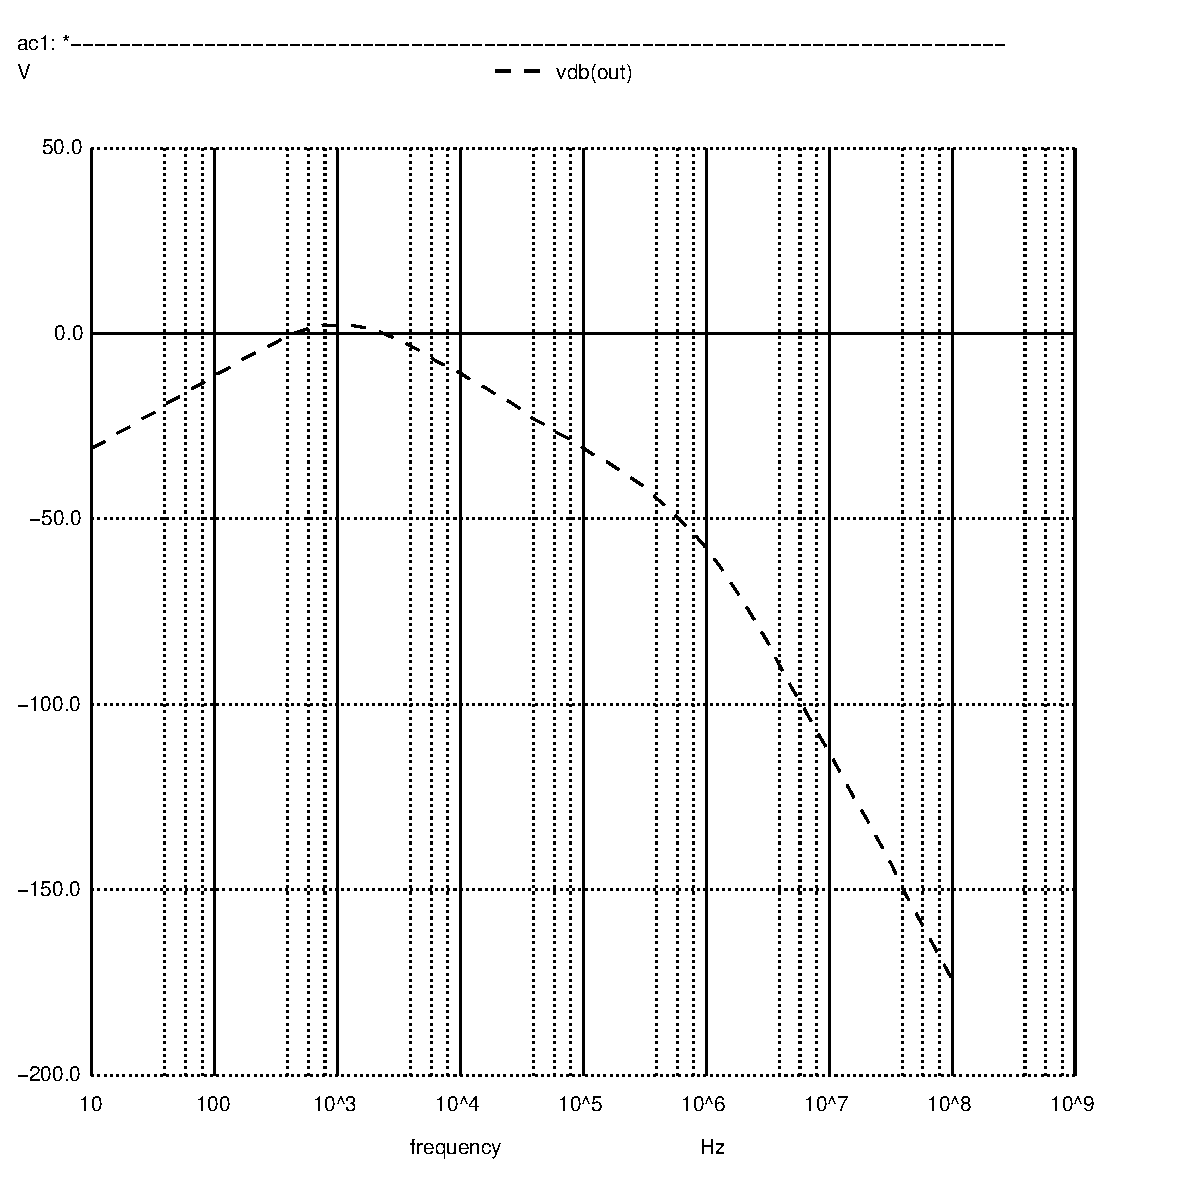
\includegraphics[width=0.6\textwidth]{vo1f}
\caption{Frequency response - gain}
\end{figure}

\begin{figure}[H]
\centering
\includegraphics[width=0.6\textwidth]{vo1f_phase}
\caption{Frequency response - phase}
\end{figure}

\subsection{Optimized circuit}
